 \documentclass{journal}[IEEEtran, twocolumn]             % No modificar

% PASO 1. Reemplace "Práctica 1" por el número de la práctica que corresponda
\newcommand{\dochead}{Practice N°1}     

% PASO 2. Verifique el título de la práctica corresponda.
\newcommand{\docsubhead}{GNU Radio and SDR}  

% PASO 3. Reemplace "B1A - 02" por el grupo de la asignatura y el número de su grupo de laboratorio
\newcommand{\teamname}{B2}     

% PASO 4. OPCIONAL: Reemplace "\docsubhead \docsubhead" por el título del documento en caso de requerirse.
\newcommand{\titulo}{\dochead: \docsubhead}      

% PASO 5. Reemplace "31 de diciembre de 2030" por la fecha de su documento
\newcommand{\fecha}{February 17, 2024}      

% To load packages
\usepackage{microtype}
\usepackage[T1]{fontenc}
\usepackage[utf8]{inputenc} 
\usepackage[english]{babel}
\usepackage[letterpaper,left=2.0cm,top=2.0cm,right=2.0cm,bottom=4.0cm]{geometry}
\usepackage{amsmath}
\usepackage{amsfonts}
\usepackage{fancyhdr}
\usepackage{fancyvrb}
\usepackage{listings}
\usepackage{array}
\usepackage{graphicx,color,enumerate}	
\usepackage{multirow} 
\usepackage{multicol}
\usepackage{authblk}
\usepackage{charter}    
\usepackage{titling}
\usepackage{url}
\usepackage{hyperref}
\usepackage{xcolor}
\usepackage{tabularx}
\usepackage{tikz}
\usepackage{float}
\usepackage{booktabs}
\usepackage{longtable}
\usepackage{adjustbox}
\usepackage{subcaption}
\usepackage{colortbl}
\usepackage{tcolorbox}

\definecolor{uisgreen}{RGB}{125,194,3}
\definecolor{gray97}{gray}{.97}
\definecolor{gray75}{gray}{.75}
\definecolor{gray45}{gray}{.45}

\setlength{\droptitle}{-1.8cm}
\pagestyle{fancy}

%%% Header definition
\headheight=60pt 						% header height 
\renewcommand{\headrulewidth}{4pt}
\let\oldheadrule\headrule% Copy \headrule into \oldheadrule
\renewcommand{\headrule}{\color{uisgreen}\oldheadrule}

\fancyhead[L]							% left header 
{	\begin{minipage}{2.5cm}
		
\includegraphics[scale=0.3]{./figs/uislogohoriz.png} 
	\end{minipage}	
	\begin{minipage}{5cm}
	    \color{uisgreen}
	    \footnotesize {\textsf{Universidad Industrial de Santander\\ 
				Escuela de Ingenierías Eléctrica, \\
				Electrónica y de Telecomunicaciones	}}	
	\end{minipage}
}
\fancyhead[R] { 							%la "C" indica al centro
	\begin{minipage}{8cm}
	    \color{uisgreen}
	    \begin{flushright}
    	    \small{\textsf{Communications II - LAB (27145)}} \\
            \normalsize{\textsf{\dochead: \textbf{\docsubhead}}} \\
    	    \small{\textsf{Group: \textbf{\teamname}}}
	    \end{flushright}
    \end{minipage}
    \begin{minipage}{1.2cm}
		
\includegraphics[width=1.0\textwidth]{./figs/logoE3T.png} 
	\end{minipage}	
}
%%% End header definition

\lstset{ frame=Ltb,
     framerule=0pt,
     aboveskip=5pt,
     framextopmargin=3pt,
     framexbottommargin=3pt,
     framexleftmargin=0.4cm,
     framesep=0pt,
     rulesep=.4pt,
     backgroundcolor=\color{gray97},
     rulesepcolor=\color{black},
     %
     stringstyle=\ttfamily\color{red!50!brown},
     showstringspaces = false,
     basicstyle=\small\ttfamily,
     commentstyle=\color{gray45},
     keywordstyle=\color{blue}\bfseries,
     %
     numbers=left,
     numbersep=5pt,
     numberstyle=\tiny,
     numberfirstline = false,
     breaklines=true,
   }

% minimizar fragmentado de listados
\lstnewenvironment{listing}[1][]
   {\lstset{#1}\pagebreak[0]}{\pagebreak[0]}

\lstdefinestyle{consola}
   {basicstyle=\scriptsize\bf\ttfamily,
    backgroundcolor=\color{gray75},
   }

\lstdefinestyle{C}
   {language=C,
   }

             % No modificar


\begin{document}                    % No modificar

\title{\textbf{\titulo}}            % No modificar

% PASO 6. Agregar aquí el nombre y código de los autores.  
\author{
Jeanpaull Valencia Quintero - 2200496 \\
Ramon Stiven Sarmiento Castro - 2200503 \\
Juan Manuel Tellez Calderon - 2194235
}

\affil{\small{Escuela de Ingenierías Eléctrica, Electrónica y de Telecomunicaciones} \\ % No modificar
\small{Universidad Industrial de Santander}} % No modificar

\date{\fecha}                       % No modificar

\maketitle                          % No modificar
\thispagestyle{fancy}               % No modificar

%---------------------------------------------------------------
% PASO 7. **..**...****INICIE SU DOCUMENTO DESDE AQUI***...**...
%%%%% A PARTIR DE AQUÍ EDITE EL DOCUMENTO PARA AGREGAR TODO EL CONTENIDO REQUERIDO PARA EL ENTREGABLE CORRESPONDIENTE
%%%%  Todo el contenido a partir de este punto es SOLAMENTE ILUSTRATIVO.

\color{black}

\begin{multicols}{2}

\begin{abstract}
    In this practice, the concepts of GIT and GNURadio are used. Specifically, the practice aims to demonstrate the use of branches in GitHub in order to showcase version control. Regarding GNURadio, the goal is to put into practice the construction of blocks using the Python programming language, while applying concepts associated with digital communications, such as the use of time averages, as well as more basic blocks in the context of signals, such as the accumulator and differentiator.

\end{abstract}

\section{Methodology}
The methodology used is divided into 2 main elements:

\begin{itemize}
    \item Use of GIT and branch planning.
    \item Construction and use of blocks in GNURadio.
\end{itemize}

\subsection{GIT}
The objective of GIT in this case was version control. In this scenario, the construction of independent branches was carried out so that each member could work on one or several predetermined sections of the activity, such as the Report or the construction of blocks in GNURadio. The following procedure was followed:

\begin{enumerate}

    \item The main branch is cloned, which serves as our template. From this, branches of the same hierarchy are created with the content of main, done through the web page.
    
    \item Each participating student is assigned a branch from the independent branches to upload the divided content.
    
    \item  Upon completion of the GNURadio activity and the Report, the respective files are saved using the 'commit' and 'push' actions.
    
    \item Finally, a merge of the contents of each branch is performed to generate a single branch with all the content, done through the 'merge' action."
\end{enumerate}

Fig \ref{fig:fig_1} shows how the branches work.

    \begin{figure}[H]
        \centering
        \begin{adjustbox}{frame=1pt 1pt,center=1pt}
            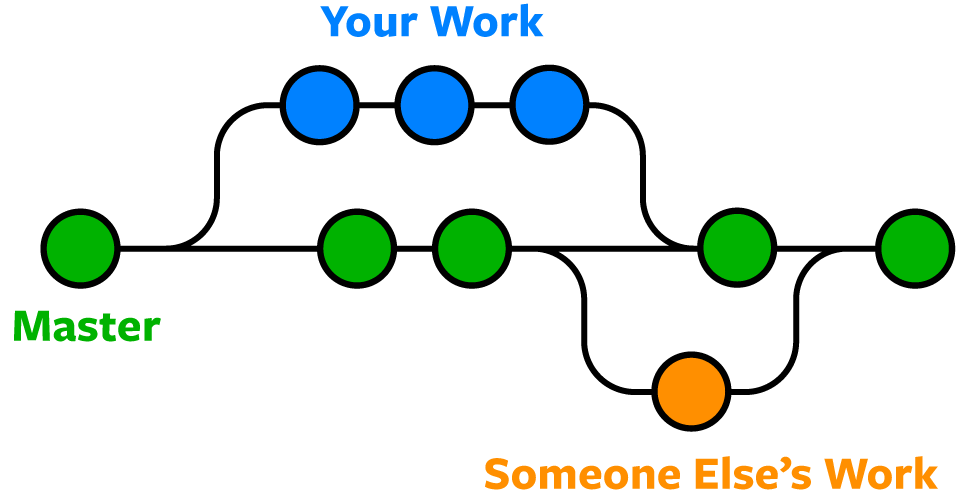
\includegraphics[width=0.3\textwidth]{figs/branch.png}
        \end{adjustbox}
        \caption{\centering Use of branches in Github}
        \label{fig:fig_1}
    \end{figure}

\subsection{GNURadio}

As for the GNURadio process, the development of the accumulator, difference, and averages blocks was undertaken. The associated process is related to building blocks based on the guidance provided in the GNURadio wiki. Thus, the construction process was divided into:

\begin{enumerate}

\item Blocks are constructed based on other reference blocks, written in Python. Some corrections are made to the given code to ensure correct results.
\item The blocks are applied based on the application. In this case, the use of accumulator and differentiator blocks in a discrete signal or pulse context is suggested, using a test vector.
\item Additionally, the time averages block is applied to demonstrate a real-world example. In this case, the time averages block is used for the following cases: (Mean, root mean square, standard deviation, RMS value, and average power).

\end{enumerate}
    
\section{Results and analysis}

The results obtained from this practice consist of the following:

\begin{enumerate}
    \item  Application of accumulator and differentiate blocks.
    \item  Usage of time averages block.
\end{enumerate}

\subsection{Accumulate and differentiate blocks}
Both of the blocks were implemented in the same project, as shown in figure \ref{fig:fig_2}

\begin{figure}[H]
        \centering
        \begin{adjustbox}{frame=1pt 1pt,center=1pt}
            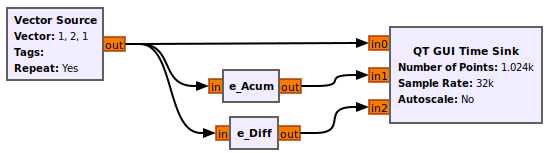
\includegraphics[width=0.8\columnwidth]{figs/blocks.png}
        \end{adjustbox}
        \caption{\centering Implementation of block Accumulate and Differentiate in GNU Radio}
        \label{fig:fig_2}
\end{figure}

The following is the code used for the block, and a brief explanation of how it works

\subsubsection{Accumulate block}
The accumulator block works as a summation where the upper limit of the summation is the position of the output vector.

\begin{equation*}
    y[n] = \sum_{i=0}^{n} x[i]
\end{equation*}

\subsubsection{Differentiate block}
The differentiator block works in the same way as the accumulator, but it is no longer an addition but a succession of subtractions, so they are accumulated subtractions.

\begin{equation*}
    y[n] = x[n] - y[n-1]
\end{equation*}

Finally, figure \ref{fig:fig_3} shows an example of the project in gnu radio with each block, where the periodic input signal is $x = [1,2,1]$.

\begin{figure}[H]
        \centering
        \begin{adjustbox}{frame=1pt 1pt,center=1pt}
            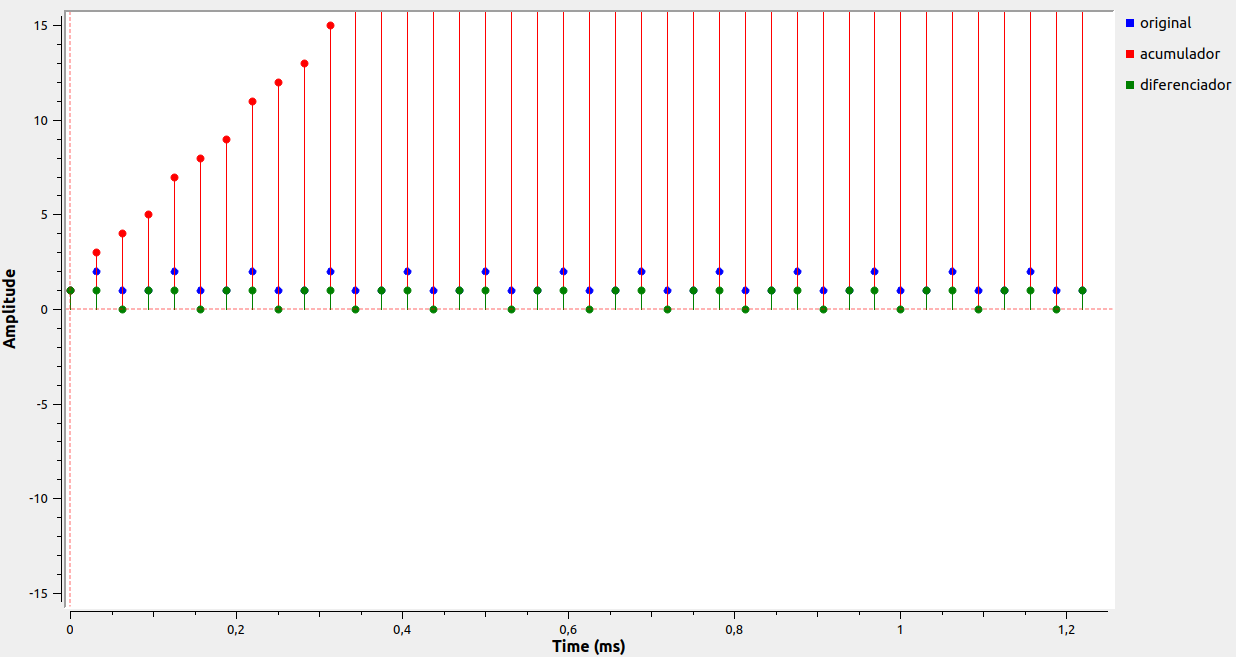
\includegraphics[width=1\columnwidth]{figs/ex_acum_diff.png}
        \end{adjustbox}
        \caption{\centering Example using the blocks}
        \label{fig:fig_3}
\end{figure}

\subsection{Time averages block}
The time averages block basically implements all the calculations that could be observed in class, such as the mean, the root mean square, the RMS value, the average power, and the standard deviation. In this case, all these operators are encoded in a single block, resulting in the output shown in Figure \ref{fig:fig_4}.


\begin{figure}[H]
        \centering
        \begin{adjustbox}{frame=1pt 1pt,center=1pt}
            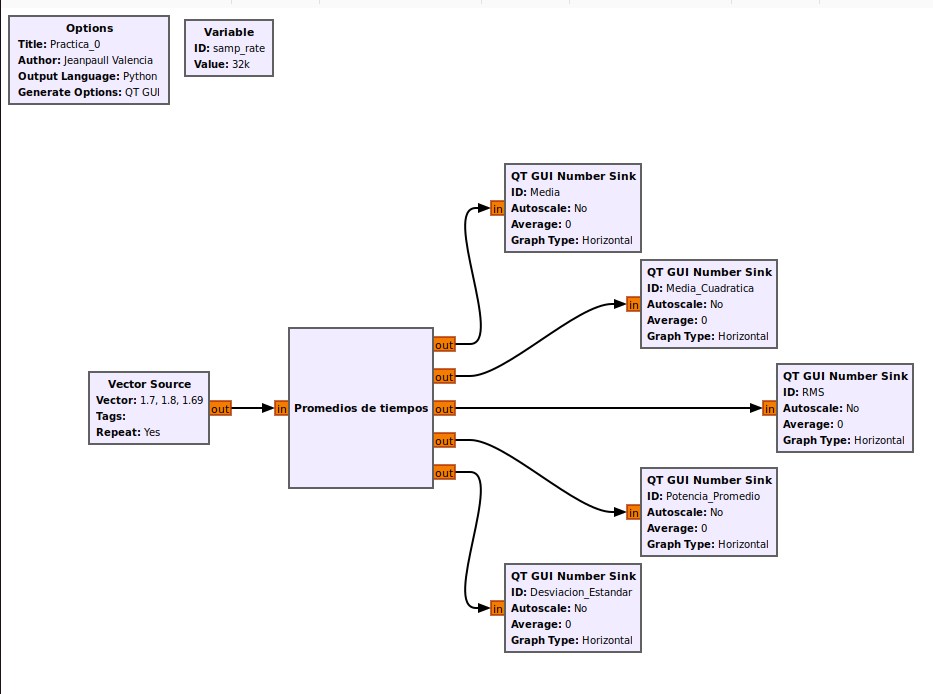
\includegraphics[width=0.8\columnwidth]{figs/time_averages.png}
        \end{adjustbox}
        \caption{\centering Implementation of an averages block in GNU Radio}
        \label{fig:fig_4}
\end{figure}

El bloque contiene las siguientes formulas:

\subsubsection{Media}

 The mean allows us to obtain the most representative value of the sample distribution.

\begin{equation*}
\left \langle x[n] \right \rangle = \lim_{N\rightarrow \infty }\frac{1}{N}\sum_{i = 1}^{N}x[i]
\end{equation*}

\subsubsection{Media cuadrática}

The mean square allows us to obtain a value similar to the mean, but comparable in the case of encountering negative values in our samples, since in many cases we may encounter a mean of 0.

\begin{equation*}
    x_{C} = \left \langle |x[n]|^{2} \right \rangle
\end{equation*}

\subsubsection{Valor RMS}

The RMS value has the same properties; however, it provides us with a result comparable with the initial units of the samples taken. It also allows us to obtain an expected value of a waveform that encapsulates all its behavior.

\begin{equation*}
    X_{RMS} = \sqrt{\left \langle |x[n]|^{2} \right \rangle}
\end{equation*}

\subsubsection{Potencia promedio}

Average power allows us to obtain a bounded range of values, in this case, 'Energy'. It could also be abstractly related as variation, because in the context of electrical and electronic engineering it leads to a result more associated with signal intensity.

\begin{equation*}
    P = X_{RMS}^{2}
\end{equation*}

\subsubsection{Desviación estándar}

The standard deviation allows us to understand the variation of our signal or samples with respect to the mean, with units comparable to those of the input vector.

\begin{equation*}
    \sigma_{x} = \sqrt{\left \langle |x[n]-x_{m}|^{2} \right \rangle}
\end{equation*}

\subsubsection{Application example}

\begin{figure}[H]
        \centering
        \begin{adjustbox}{frame=1pt 1pt,center=1pt}
            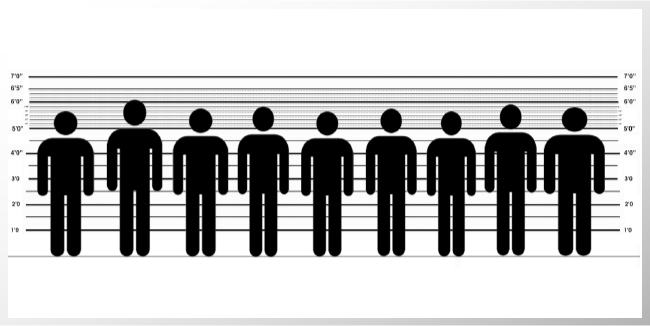
\includegraphics[width=0.8\columnwidth]{figs/height.png}
        \end{adjustbox}
        \caption{\centering Experiment involving people's height}
        \label{fig:fig_5}
\end{figure}

In this case, a random experiment was used based on the heights of people in a basketball set (Figure \ref{fig:fig_5}). Since basketball is a fairly popular sport, heights generally range above 1.8m. But how does Colombia fare in this regard? We can observe this in the following example applied to the time averages block. For this, a database of 11 basketball players from the Colombian professional league was consulted, from which the following input vector was obtained:

\begin{equation*}
    x[n] = [1.96,1.98,1.88,1.85,2.01,1.96,1.98,1.99,2.13,1.75,2.05]
\end{equation*}

A partir de estos datos se hace uso de las ecuaciones estadísticas antes mencionadas, lo cual da lo siguiente observado en la figura \ref{fig:fig_6}.

\begin{figure}[H]
        \centering
        \begin{adjustbox}{frame=1pt 1pt,center=1pt}
            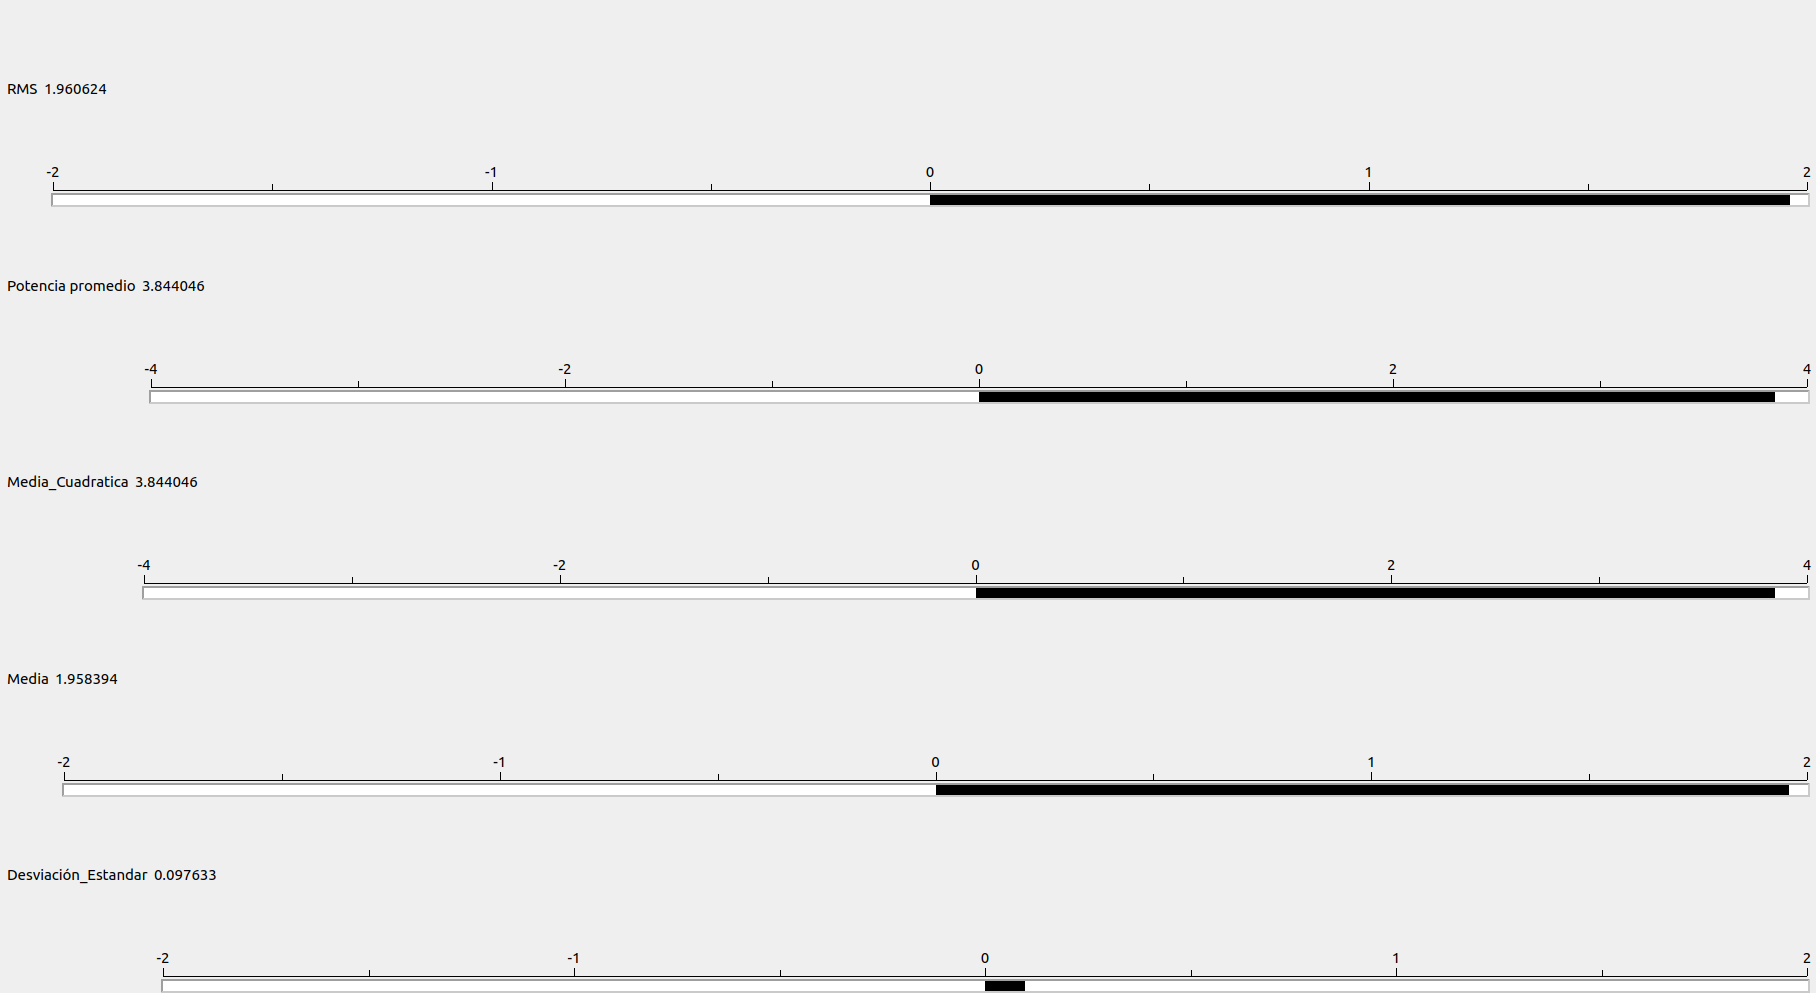
\includegraphics[width=0.8\columnwidth]{figs/T_A_results.png}
        \end{adjustbox}
        \caption{\centering Experiment involving people's height}
        \label{fig:fig_6}
\end{figure}

In this case, we obtain a similar RMS value and mean. Why is this? This is basically because both have a set of positive samples. Therefore, as mentioned above, the RMS value is a way of measuring the concentration of values in a function while maintaining the same units. However, since the range of values is positive, the mean and RMS value are approximately, if not identical.

The average power in this context, since it is not talking about energy, has a meaning more associated with how much the samples are related to other human height events. Therefore, its context is not so relevant.

\section{Conclusions}

\begin{enumerate}
    \item Time averaging analysis of a signal can show us its trends, as demonstrated in the example of heights, where the mean and RMS values told us what the highest coincidence in heights was. Thus, in the context of other signals, they also allow us to know their trends and the way in which they are transmitted.
    \item Version control applications allow you to track and monitor changes in collaborative projects. In addition, these tools help to create a more professional work environment.
\end{enumerate}

\section{Anexes}
In the following link you will find the codes that were used in this first practice: 
\begin{itemize}
    \item \url{https://github.com/RamonSsc/ComunicationII_2024_1-RJT/tree/main/Practica1}
\end{itemize}

% NO MODIFIQUE NI ELIMINE ESTA PARTE PARA QUE  APAREZCAN LAS REFERENCIAS
\bibliographystyle{IEEEtran}
\bibliography{bibliografia.bib}\nocite{*}

\end{multicols}
\end{document}